
\begin{tikzpicture}[
    grow=down,
    level 1/.style={sibling distance=3.5cm,level distance=2.2cm},
    level 2/.style={sibling distance=3.5cm, level distance=2.2cm},
    edge from parent/.style={draw=gray},
    edge from parent path={(\tikzparentnode.south) -- (\tikzchildnode.north)},
    kant/.style={text width=2cm},
    every node/.style={text ragged, inner sep=2mm},
    punkt/.style={rectangle, top color=white, bottom color=white, draw=black }
    ]

\node[punkt, text width=5.5em] {$initial\ \mathcal{K}$}
    %Lower part lv1
    child {
        node[punkt] [rectangle split, rectangle split, rectangle split parts=1,
         text ragged] { $\texttt{S:= S},x\approx\epsilon$  }
                             child{
                             	node { $\texttt{unsat}$}
                             	edge from parent node[kant, above, pos=.6] {$\texttt{A-Conflict}$}
                             }                    
        edge from parent
            node[kant] {$\texttt{Len-Split}$}
    }
    child {
            node[punkt] [rectangle split, rectangle split, rectangle split parts=1,text ragged] { $\texttt{A:= A},\texttt{len}\ x > 0$  }
            child {
              node[punkt] [rectangle split, rectangle split, rectangle split parts=1,text ragged] { $\texttt{S:= S},z\approx\epsilon$  }
              child{
               	node { $\texttt{unsat}$}
               	edge from parent node[kant, above, pos=.6] {$\texttt{A-Conflict}$}
              }
              edge from parent node[kant, below, pos=.6] {$\texttt{Len-Split}$}
            }
            child {
               node[punkt] [rectangle split, rectangle split, rectangle split parts=1,text ragged] { $\texttt{A:= A},\texttt{len}\ z > 0$  }
               child{
                  node[punkt] [rectangle split, rectangle split, rectangle split parts=1,text ragged] { $\texttt{S:= S},y\approx\epsilon$  }
                  child{
                    node { $\texttt{unsat}$}
                    edge from parent node[kant, above, pos=.6] {$\texttt{A-Conflict}$}
                  }
                  edge from parent node[kant] {$\texttt{Len-Split}$}
               }
               child{
                  node[punkt] [rectangle split, rectangle split, rectangle split parts=1,text ragged] {$\texttt{A:= A},\texttt{len}\ y > 0$}
                  child{
                    node[punkt] [rectangle split, rectangle split, rectangle split parts=1,text ragged] {$\texttt{F:= F},con(x,l_1,z)\mapsto (x,l_1,z),con(y,l_2,z)\mapsto(y,l_2,z)$}
                    edge from parent node[kant] {$\texttt{N-Form2,F-Form2,N-Form1,F-Form1}$}
                  }                  
                  edge from parent node[kant] {$\texttt{Len-Split}$}
               }
               edge from parent node[kant, below, pos=.6] {$\texttt{Len-Split}$}
            }            
            edge from parent node[kant, below, pos=.6] {$\texttt{Len-Split}$}
        }
    %Upper part, lv1
;
\end{tikzpicture}

\begin{center}
\Tree 
[.{$ initial \ \mathcal{K} ::  \texttt{Len-Split}$  } 
	[
		.{ $\texttt{S:= S},x\approx\epsilon :: \texttt{S-Conflict}$  }
		{ $\texttt{unsat}$  }
	]
	[
		.{ $\texttt{A:= A},\texttt{len}\ x > 0$  }					 
	]
]
\end{center}


\begin{figure}
\centering
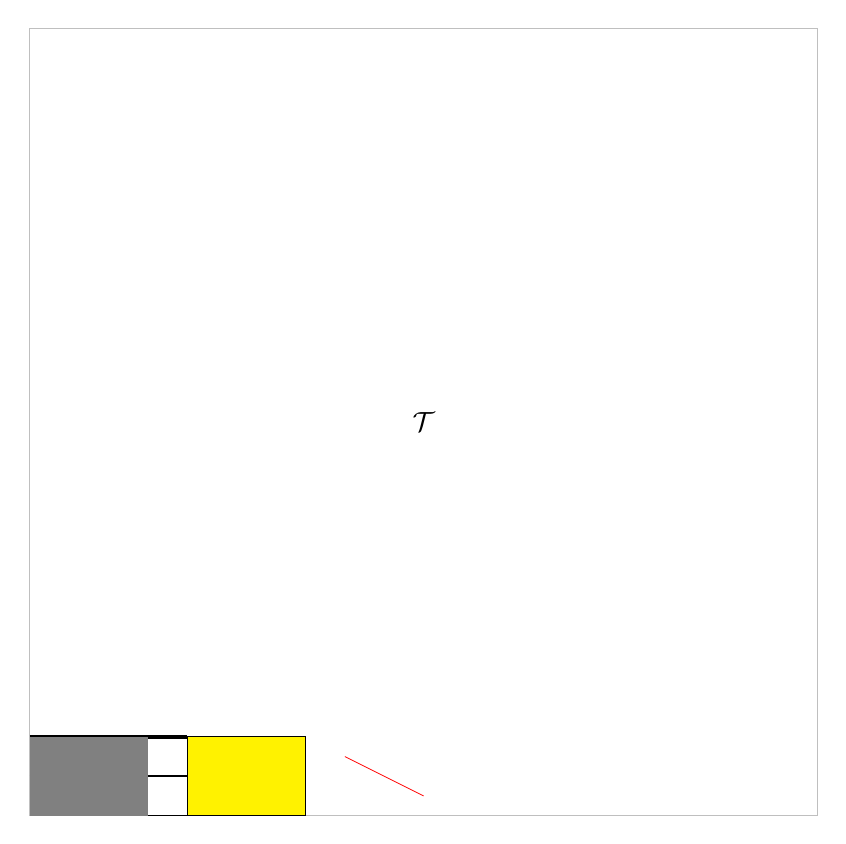
\begin{tikzpicture}
\draw [lightgray](0,0) --(0,10) -- (10,10)-- (10,0) --(0,0);
\draw [ultra thick] (0,1) -- (2,1);
\draw [thick] (0,0.5) -- (2,0.5);
\draw [thin] (0,0) -- (2,0);
\draw [line width=0.01cm, red] (4,.75) -- (5,.25);
\path [fill=gray] (0,0) rectangle (1.5,1);
\draw [fill=yellow] (2,0) rectangle (3.5,1);
\node at (5,5) {$ \mathcal{T} $};
\end{tikzpicture}
\caption{The derivation tree for example 1.}
\end{figure}


\begin{figure}
\centering
\begin{tikzpicture}
\draw [lightgray](0,0) --(0,10) -- (20,10)-- (20,0) --(0,0);

\draw [->] (5,5) -- (4,4.5);
\node [right] at (2,8) {$\texttt{F:= F},\texttt{con}(x,l_1,z)\mapsto (x,l_1,z),\texttt{con}(y,l_2,z)\mapsto(y,l_2,z)$};
\node [right] at (6,7.2) {$\texttt{F-Unify}$};
\draw [->] (6,7.8) -- (6,6.8);
\node [right] at (5,6.5) {$\texttt{S:= S},x\approx y$};

\end{tikzpicture}
\caption{The derivation tree for example 1.}
\end{figure}

\begin{figure}
\centering
\begin{tikzpicture}
\draw [lightgray](0,0) --(0,10) -- (20,10)-- (20,0) --(0,0);

\node [below] at (10,10) {$ initial \ \mathcal{K}$};
\node [below] at (10,9.6) {$\texttt{Len-Split}$};

\draw [->] (10,9.3) -- (8,8.5);
\draw [->] (10,9.3) -- (12,8.5);


\draw [->] (5,5) -- (4,4.5);
\node [right] at (2,8) {$\texttt{F:= F},\texttt{con}(x,l_1,z)\mapsto (x,l_1,z),\texttt{con}(y,l_2,z)\mapsto(y,l_2,z)$};
\node [right] at (6,7.2) {$\texttt{F-Unify}$};
\draw [->] (6,7.8) -- (6,6.8);
\node [right] at (5,6.5) {$\texttt{S:= S},x\approx y$};

\end{tikzpicture}
\caption{The derivation tree for example 1.}
\end{figure}


